\subsection{Finding transfer functions}

\begin{figure}[h!]
    \centering
    \includegraphics[scale=0.4]{roll_loop_no_i.PNG}
    \caption{Roll loop without integrator}
    \label{fig:roll}
\end{figure}

Let's look at the innermost loop, the roll loop, and derive the expression for $H_{\phi/\phi_c}$ using figure \ref{fig:roll}.
\begin{equations}
    \begin{gather*}
        s \phi = ((\phi_c - \phi) k_{p_\phi}- k_{d_\phi}s \phi) \frac{a_{\phi_2}}{s + a_{\phi_1}} \\
        \Rightarrow (s + \frac{k_{p_\phi}a_{\phi_2}}{s + a_{\phi_1}} + \frac{ sk_{d_\phi}a_{\phi_2}}{s + a_{\phi_1}} ) \phi = (\frac{k_{p_\phi}a_{\phi_2}}{s + a_{\phi_1}})\phi_c \\
        \Rightarrow H_{\phi/\phi_c}(s)  = \frac{(\frac{k_{p_\phi}a_{\phi_2}}{s + a_{\phi_1}})}{ (s + \frac{k_{p_\phi}a_{\phi_2}}{s + a_{\phi_1}} + \frac{ sk_{d_\phi}a_{\phi_2}}{s + a_{\phi_1}} )}  
        = \frac{k_{p_\phi}a_{\phi_2}}{s^2 + s(a_{\phi_1} + k_{d_\phi} a_{\phi_2}) + k_{p_\phi}a_{\phi_2}} \\
    \end{gather*}
\end{equations}
 \begin{figure}[h!]
     \centering
     \includegraphics[scale=0.35]{system_loop.PNG}
     \caption{System loop}
     \label{fig:system}
 \end{figure}

To find the course transfer function, we will use figure \ref{fig:system}. Note that we cannot approximate the inner loop this time. 
\begin{equations}
    \begin{align*}
    \chi &= \frac{g}{V_gs}(d_\chi + \phi)  \\
    \phi &= \frac{1}{s} ((\phi_c - \phi) k_{p_\phi}- k_{d_\phi}s \phi) \frac{a_{\phi_2}}{s + a_{\phi_1}} \\
    \phi_c &= (\chi_c - \chi)(\frac{k_{i_\chi}}{s} + k_{p_\chi}) \\
    \Rightarrow \chi &= \frac{g}{V_gs}(d_\chi + ( \frac{1}{s} (((\chi_c - \chi)(\frac{k_{i_\chi}}{s} + k_{p_\chi}) - \phi) k_{p_\phi}- k_{d_\phi}s \phi) \frac{a_{\phi_2}}{s + a_{\phi_1}})) 
    \end{align*} 
\end{equations}
Let $d_\chi = 0.$
\begin{equations}
    \begin{align*}
        \frac{V_g s(s^2 + sa_{\phi_1})}{g a_{\phi_2}} \chi &= \frac{k_{p_\phi} k_{i_\chi} + k_{p_\phi} k_{p_\chi}s}{s}\chi_c - \frac{k_{p_\phi} k_{i_\chi} + k_{p_\phi} k_{p_\chi}s}{s} \chi + (-1-k_{d_\phi}s)\phi \\
        \chi &= \frac{((k_{p_\phi} k_{i_\chi} + k_{p_\phi} k_{p_\chi}s) ga_{\phi_2} ) \chi_c + (ga_{\phi_2}(-1-k_{d_\phi}s)) \phi }{V_g s^4 + V_g a_{\phi_1}s^3  + ga_{\phi_2}k_{p_\phi} k_{p_\chi}s+ ga_{\phi_2}k_{p_\phi} k_{i_\chi}}
    \end{align*}
\end{equations}

Because of the super position principle we know 
\begin{equation*}
    H_{\chi/\chi_c} = \frac{(k_{p_\phi} k_{i_\chi} + k_{p_\phi} k_{p_\chi}s) ga_{\phi_2} }{V_g s^4 + V_g a_{\phi_1}s^3  + ga_{\phi_2}k_{p_\phi} k_{p_\chi}s+ ga_{\phi_2}k_{p_\phi} k_{i_\chi}}
\end{equation*}












\begin{figure}[H]
    \centering
    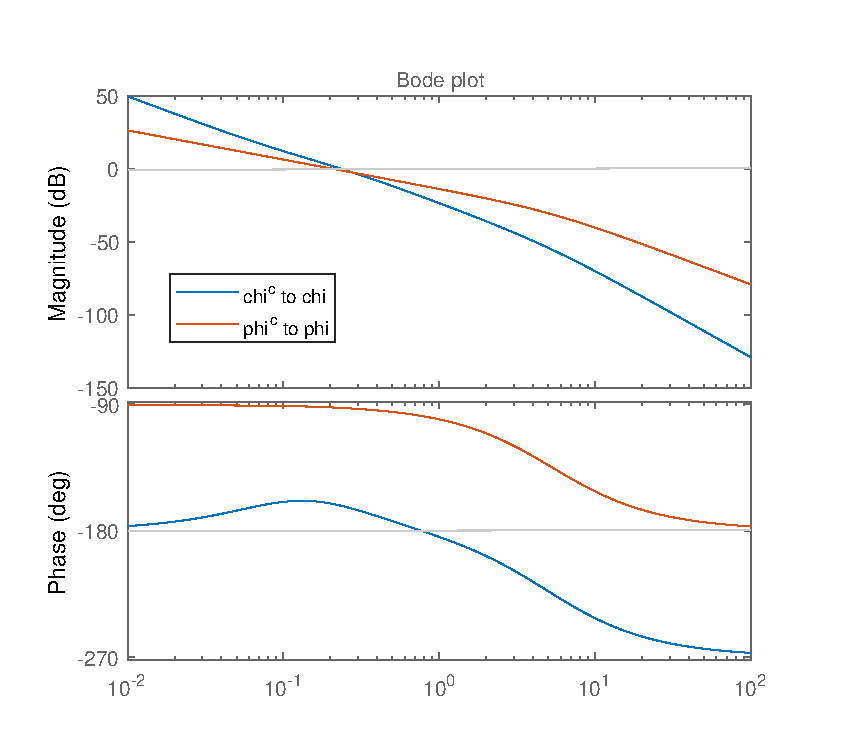
\includegraphics[scale = 0.7]{bode.eps}
    \caption{Bode plot whit different natural frequencies. }
    \label{bode}
\end{figure}

\begin{figure}[H]
    \centering
    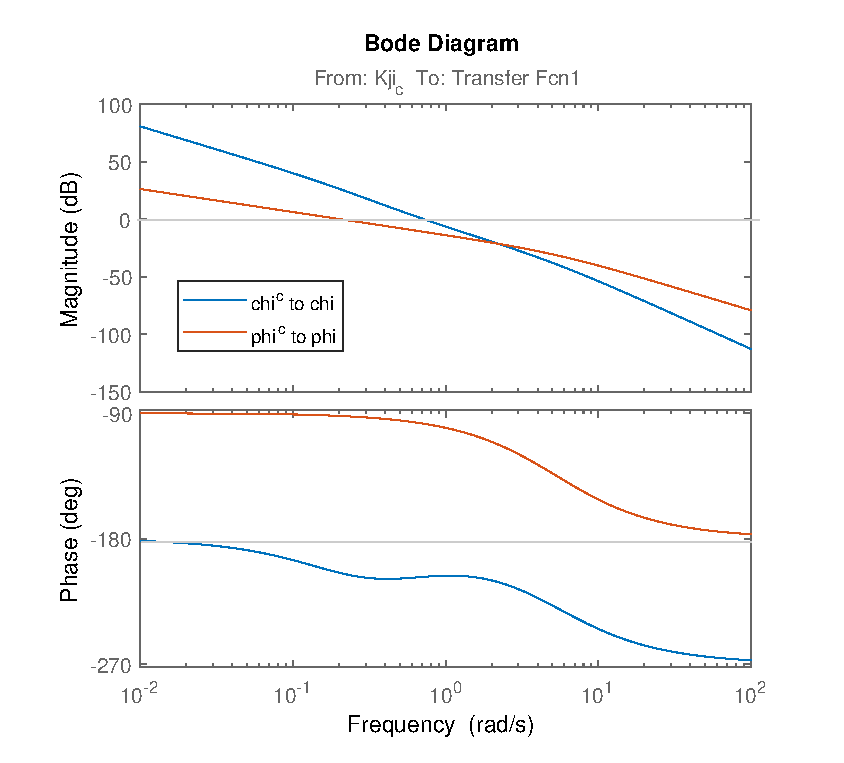
\includegraphics[scale = 0.7]{bode_2.eps}
    \caption{Bode plot whit equal natural frequencies.}
    \label{bode_2}
\end{figure}

We see from the bode plot in figure(\ref{bode}) that the two systems are stable. $\omega_c$ is in both cases lower than $\omega_{180}$. This is because we chose a natural frequency 6 times lower for the course loop than the roll loop. If we had chosen the same natural frequency for both loops, we would get the bode plot in figure(\ref{bode_2}). In this case, we see that the the transfer function from $\chi^c$ to $\chi$ is not stable because its phase is smaller than $-180 deg$ for all frequencies. This is because the roll loop is as slow as the course loop. The roll loop needs to be faster so that the course loop can assume that the roll loop has reached a stationary value.